\section{Analysis}

\begin{theorem}(Bolzano\footnote{\textsc{Bernard Bolzano} (1781 -- 1848), Bohemian mathematician and Catholic priest.}-Weierstrass\footnote{\textsc{Karl Weierstrass} (1815 -- 1897), German mathematician, \enquote{father of modern analysis}.})\label{thrm:bolzano_weierstrass}
	Let $\seq[x_n]$ be a bounded sequence of real numbers, then $\seq[x_n]$ has a convergent subsequence.
\end{theorem}

\begin{proof}[Proof \cite{src:bolzano_weierstrass}]
	Let $\seq[x_n]$ be a bounded sequence of real numbers, i.e. there exists an $L\in\mathbb R$ s.t. $\abs{x_n}\leq L$ for all $n\in\mathbb N$. We now proceed in several steps to construct a convergent subsequence of $\seq[x_n]$.
	
	\textit{Step 1}: Set $a_0 := -L$ and $b_0 := L$. Clearly, $\abs{b_0 - a_0} = 2L$. We now divide the interval $[a_0, b_0]$ into two halves. At least one half contains infinitely many sequence elements. We now pick that half and denote it by $[a_1, b_1]$. Clearly, either $a_1 = a_0$ or $b_1 = b_0$. Also, $\abs{b_1 - a_1} = \abs{b_0 - a_0}/2 = L$ and $[a_1, b_1]\subset [a_0, b_0]$. Figure \ref{fig:bolzano_weierstrass} visualizes this. 
	\begin{figure}[h!]
		\centering
		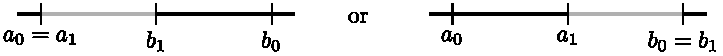
\includegraphics[width=0.7\textwidth]{Figures/bolzano_weierstrass_interval_construction.pdf}
		\caption{Construction of subsequence of $\seq[x_n]$.}
		\label{fig:bolzano_weierstrass}
	\end{figure}
	Since there are infinitely many sequence elements in $[a_1, b_1]$, we can choose a sequence element contained in $[a_1, b_1]$, which we denote by $x_{n_1}$. 
	
	We can now characterize the search procedure inductively: For $k\in\mathbb N$, let $[a_k, b_k]$ be s.t. $[a_k, b_k]$ contains infinitely many sequence elements of $\seq[x_n]$, $[a_k, b_k]\subset [a_{k-1}, b_{k-1}]$ and $\abs{b_k - a_k} = 2L/2^k = L/2^{k-1}$. Then we construct $[a_{k+1}, b_{k+1}]$ by dividing $[a_k, b_k]$ into two halves and choosing the half that contains infinitely many sequence elements, i.e. either $a_{k+1} = a_k$ or $b_{k + 1} = b_{k}$. Clearly, $\abs{b_{k+1} - a_{k+1}} = \abs{b_k - a_k}/2 = L/2^{k}$. Since $[a_{k+1}, b_{k+1}]$ contains infinitely many sequence elements, we can choose an $x_{n_{k+1}}\in [a_{k+1}, b_{k+1}]$ s.t. $x_{n_{k+1}} > x_{n_k}$. In this way, we generate nested intervals of the form 
	\[
		\underbrace{[a_0, b_0]}_{\text{length } 2L} \supset \overbrace{\underbrace{[a_1, b_1]}}^{x_{n_1}\in}_{\text{length } L} \supset \overbrace{\underbrace{[a_2, b_2]}}^{x_{n_2} \in }_{\text{length }L/2} \supset \cdots		
	\]
	
	\textit{Step 2}: The sequence $\seq[a_n]$ is monotonically increasing and bounded above by $b_0$, so by Corollary \ref{corollary:mono_inc_real_seq_convergence}, it converges to an $x\in\mathbb R$.
	
	\textit{Step 3}: We now show that $\left(x_{n_k}\right)_{k\in\mathbb N}$ converges to $x$. For this, note that
	\[
		\abs{x_{n_k} - x} \leq \abs{x_{n_k} - a_{k}} + \abs{a_k - x} \leq \frac{L}{2^{k-1}} + \abs{a_k - x} \overset{k\to \infty}{\longrightarrow} 0.
	\]
\end{proof}

\begin{corollary}[Bolzano-Weierstrass]
	Let $\seq[z_n]$ be a bounded sequence of complex numbers, then $\seq[z_n]$ has a convergent subsequence.
\end{corollary}

\begin{proof}[Proof \cite{1250430}]
	Since $\seq[z_n]$ is bounded, the real sequence $\seq[\text{Re}(z_n)]$ is also bounded, as $\abs{\text{Re}(z_n)} \leq \abs{z_n}$. Thus, $\seq[\text{Re}(z_n)]$ has a convergent subsequence, which implies that $\seq[z_n]$ has a subsequence for which the real part converges, which we denote by $\left(z_{n_k}\right)_{k\in \mathbb N}$. Since $\abs{\text{Im}(z_{n_k})} \leq \abs{z_{n_k}}$, the sequence $\left(\text{Im}(z_{n_k})\right)_{k\in\mathbb N}$ is also bounded and thus has a convergent subsequence. By Theorem \ref{thrm:seq_convergence_subsequences}, the real part of the subsequence will still converge. Therefore, there is a subsequence of $\seq[z_n]$ for which both the real and imaginary parts converge.
\end{proof}

\begin{exmp}
	Consider the real sequence $\seq[x_n]$ with $x_n := (-1)^n$, which is clearly bounded, but not convergent. However, $\seq[x_{2n}]$ and $\seq[x_{2n + 1}]$ are convergent subsequences of $\seq[x_n]$.
\end{exmp}